\documentclass[10pt]{beamer}

% Verwende etex als zugrundeliegende Implementierung (-> mehr Speicher für Tex!)
\usepackage{etex}
% Encoding
\usepackage[utf8]{inputenc}

%%% Schriften, Lokalisierung und Typographie

% T1 Schriftsystem verwenden
\usepackage[T1]{fontenc}
% LModern als Standard-Schrift
\usepackage{lmodern}
% Typographische Kleinigkeiten
\usepackage[final]{microtype}
% Fette Griechische
\usepackage{bm}

%% Lokalisierung

% Deutsche Silbentrennung
\usepackage[english]{babel}
% Deutsche Anführungszeichen
\usepackage[babel]{csquotes}

% Graphiken und Farben
\usepackage{xcolor}
\usepackage{graphicx}

% Vordefinierte Farben laden
\definecolor{jgu_rot}{RGB}{193,0,42}
\definecolor{jgu_hellgrau}{RGB}{172,172,172}
\definecolor{jgu_dunkelgrau}{RGB}{99,99,99}
\definecolor{matlab_blau}{rgb}{0.00000,0.44700,0.74100}
\definecolor{matlab_orange}{rgb}{0.85000,0.32500,0.09800}


% Tikz ist kein Zeichenprogramm!
\usepackage{tikz}
\usepackage{pgfplots}
\pgfplotsset{compat=1.12}
\usetikzlibrary{patterns}

% Standalone-Paket, damit die Tikz Bilder extern auch funktionieren
% \usepackage{standalone}

%%% Bibliographie

\usepackage[%
    backend=biber,
    style=alphabetic,
    firstinits=true
]{biblatex}


% Fix für doi2bib generierte Bibliography-Einträge
\newcommand\mathplus{+}

% kein In bei article
\renewbibmacro{in:}{%
  \ifentrytype{article}{}{\printtext{\bibstring{in}\intitlepunct}}}

% Volume und Issue no. angeben
\DeclareFieldFormat[article]{volume}{\bibstring{volume}\addnbspace #1}
\DeclareFieldFormat[article]{number}{\bibstring{number}\addnbspace #1}
\renewbibmacro*{volume+number+eid}{%
\printfield{volume}%
\setunit{\addcomma\space}%<---- was \setunit*{\adddot}%
\printfield{number}%
\setunit{\addcomma\space}%
\printfield{eid}}


%%% Grundlegende Mathematik-Pakete

% Standardpackages
\usepackage{amsmath}
\usepackage{amssymb}
\usepackage{stmaryrd}
\usepackage{mathtools}

% Bessere Ausrichtung von : vor =
\mathtoolsset{centercolon}


%%% Clevere Referenzen

\usepackage[english,noabbrev,nameinlink,capitalise]{cleveref}
\crefname{equation}{}{}

% Nummern nur für referenzierte Gleichungen
\usepackage{autonum}

% Enumerates anpassen
% \usepackage{enumitem}
% Numerierte Umgebung für Theoreme definieren
% \newlist{thmenumerate}{enumerate}{1}
% \setlist[thmenumerate]{label={\upshape(\roman*)}, align=left, widest=iii, leftmargin=*}
% \crefname{thmenumeratei}{}{}

%% Beamer Template
\usetheme{Luebeck}
\usecolortheme{beaver}


%% Navigationssymbole ausblenden
\setbeamertemplate{navigation symbols}{}

%% Seitenzahl und Gesamtanzahl in Fußleiste
\setbeamertemplate{footline}[frame number]

%% Metadaten des Dokuments
\title{First Steps towards a Reduced Basis Method for Self-Consistent Field Theory Models}
\author{Alexej Disterhoft}
\institute[Johannes Gutenberg Universität] % (optional)
{
  Institut für Mathematik\\
  Johannes Gutenberg Universität Mainz
}
\date{SoSe 2015}

%% Einzug nach Absatz und Zwischenraum
\setlength{\parindent}{0pt}
\setlength{\parskip}{8pt}

%% Mathtools
\usefonttheme[onlymath]{serif}

% restlicher Mathe-Kram
%!TEX root = main.tex

% griechisches Alphabet anpassen
\renewcommand{\epsilon}{\varepsilon}
\renewcommand{\theta}{\vartheta}


%%% Operatoren und anderes mathematisches Geplänkel

% Beträge und Normen
\DeclarePairedDelimiter{\abs}{\lvert}{\rvert}
\DeclarePairedDelimiter{\norm}{\lVert}{\rVert}

% Gauß-Klammern
\DeclarePairedDelimiter{\ceil}{\lceil}{\rceil}
\DeclarePairedDelimiter{\floor}{\lfloor}{\rfloor}

% Skalarprodukte und Duale Paarungen
\newcommand{\skprod}[2]{\left\langle#1,#2\right\rangle}
\newcommand{\Skp}[3]{\left\langle#1,#2\right\rangle_{#3}}
\newcommand{\skp}[3]{\langle#1,#2\rangle_{#3}}
\newcommand{\Dual}[2]{\left(#1,#2\right)}
\newcommand{\dual}[2]{(#1,#2)}

% Inneres und Äußeres
\newcommand{\Int}[1]{#1^\circ}
\newcommand{\Ext}[1]{\overline{#1}}

% Diverse Operatoren
\DeclareMathOperator{\spn}{span}
\DeclareMathOperator{\ee}{e}
\DeclareMathOperator{\ii}{i}
\newcommand{\Transp}{^{\mathrm{T}}}
\newcommand{\Stern}{^{*}}
\newcommand{\grad}{\nabla}
\DeclareMathOperator{\divergenz}{div}
\newcommand{\hesse}{\nabla^2}

% Einschränkung einer Funktion
\newcommand\restr[2]{\ensuremath{\left.#1\right|_{#2}}}

% Ordentlicher Befehl um Mengen zu setzen
\providecommand\given{} % so it exists
\newcommand\SetSymbol[1][]{
   \nonscript\,#1\vert\nonscript\,\mathopen{}\allowbreak}
\DeclarePairedDelimiterX\Set[1]{\lbrace}{\rbrace}{ \renewcommand\given{\SetSymbol[\delimsize]} #1 }

% Vektoren und Matrizen anders setzen
\renewcommand{\vec}[1]{\mathbf{#1}}
\newcommand{\mat}[1]{\mathbf{#1}}

% Differential-d für Integral ordentlich setzen
\newcommand*\diff{\mathop{}\!\mathrm{d}}
\newcommand*\Diff[1]{\mathop{}\!\mathrm{d^#1}}

% wesentliches Supremum
\DeclareMathOperator*{\esssup}{ess\,sup}
\newcommand\blank{{\mkern2mu\cdot\mkern2mu}}

% "Definition-Gleich"
% FIXME: deprecated
\newcommand\deq{\coloneqq}

% dichte Einbettung
% FIXME: zu hoch für Fließtext!
\newcommand\denseinclusion{\stackrel{d}{\hookrightarrow}}

% Schrift einfach anpassen
\newcommand{\changefont}[3]{
\fontfamily{#1} \fontseries{#2} \fontshape{#3} \selectfont}


%%% Textbausteine

\newcommand{\fa}{\text{für alle}~}

% um fremde Begriffe einheitlich mit Übersetzung zu setzen
\newcommand\foreign[2]{#1 \textit{#2}}


\addbibresource{literature.bib}

\begin{document}
\begin{frame}
        \titlepage
\end{frame}

\begin{frame}[t]
    \frametitle{Overarching goal}

    We want to study the phase separation behavior of polymers.

    \vfill

    \begin{columns}
        \begin{column}{0.6\textwidth}
            \begin{itemize}
                \item \onslide<2-> A \emph{polymer} is a large molecule, composed of many repeated subunits (\emph{monomers}, smaller molecules).
                \item \onslide<3-> Monomers interact with each other in and across polymers.
                \item \onslide<4-> Simplest kinds of polymers are of linear chain type.
                \item Stochastic models (e.g. random walks, ideal chain models) are used to model these.
            \end{itemize}
        \end{column}
        \begin{column}{0.4\textwidth}
            \centering
            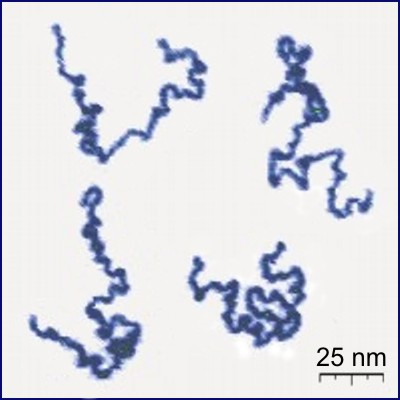
\includegraphics[width=0.9\textwidth]{figures/Single_Polymer_Chains_AFM.jpg}
        \end{column}
    \end{columns}
\end{frame}

\begin{frame}[t]
    \frametitle{Overarching goal}

    \vfill

    \begin{itemize}
        \item Polymer melts (liquid phase) can exhibit different separation behaviors:
        \onslide<2->
        \begin{itemize}
            \item \emph{macrophase separation:} liquid-liquid separation (e.g. like water / oil); mostly seen in blends of different polymers.
            \item \emph{microphase separation:} distinct ordering of individual polymer chains.
        \end{itemize}
        \onslide<3->
        \item We are interested in the microphase separation of \emph{diblock copolymers}.
        \item These consist of two types of monomers (e.g. A and B) forming two large blocks.
    \end{itemize}

    \centering
    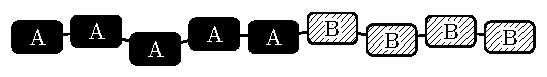
\includegraphics[width=0.8\textwidth]{figures/copoly2.pdf}
\end{frame}

\begin{frame}[t]
    \frametitle{Overarching goal}

    Several types of microphase separation observable depending on the properties of the polymers, e.g. gyroid:

    \centering
    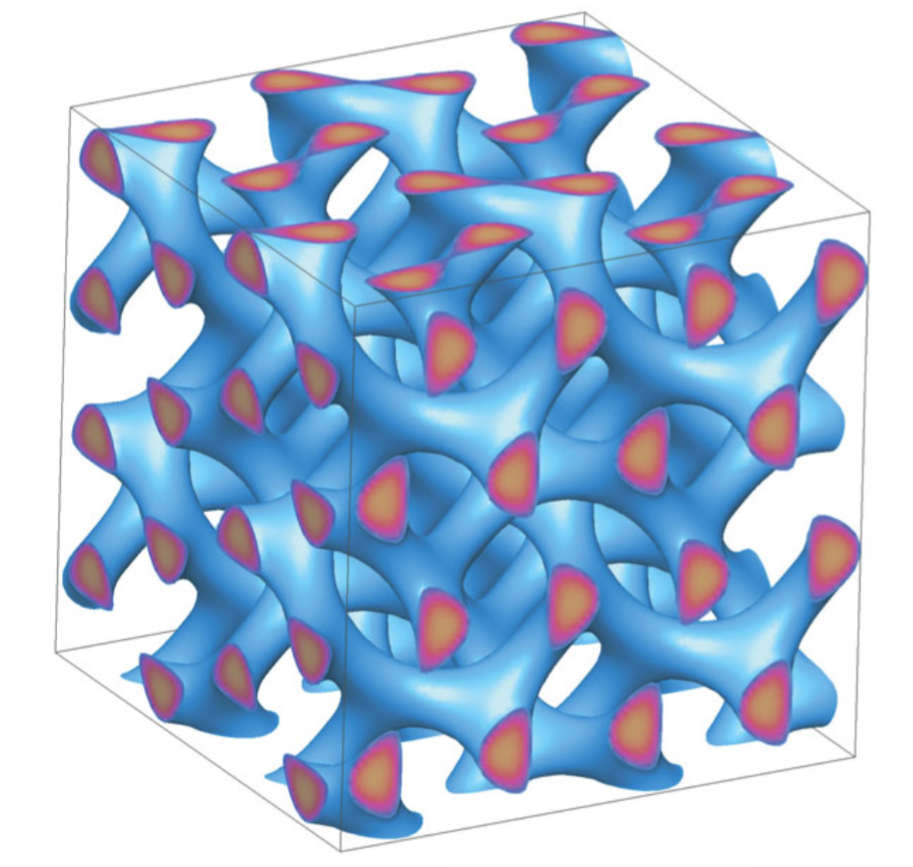
\includegraphics[scale=0.15]{figures/gyroid_separation.png}

    \onslide<2->
    Can we predict the microphase separation of polymers through theoretical models?
\end{frame}

\begin{frame}[t]
    \frametitle{So, what's self-consistent field theory?}

    Self-consistent field theory (SCFT) allows us to study the behavior of large stochastic models through simplified models.

    \vfill
    \begin{itemize}
        \item \onslide<2-> \emph{Goal:} study a complex stochastic model (e.g. a polymer melt) with a huge number of small individual interacting components (e.g. monomers).
        \item \onslide<3-> \emph{Idea:} instead of considering interactions between all the individual components, approximate the effect on a given individual by a single averaged effect (so called \emph{external field}).
    \end{itemize}

    \vfill
    \centering
    \onslide<4->
    \emph{This reduces a many-body problem to a one-body problem!}
\end{frame}

\begin{frame}[t]
    \frametitle{So, what's self-consistent field theory?}

    How can this be used?


    \begin{itemize}
        \item Model leads to a free energy functional depending on external fields $w_{A}$ and $w_{B}$, where saddle points correspond to stable microphase separations!
        \item \onslide<2-> Allows an iterative scheme that adjusts the external fields until these satisfy some saddle point equations (\emph{self consistency}).
    \end{itemize}
\end{frame}

\begin{frame}[t]
    \frametitle{So, what's self-consistent field theory?}

    Most costly part of one iteration:
    calculating a solution to the modified diffusion equation (MDE)
        \begin{equation}
            \frac{\partial}{\partial s}q(\vec{r}, s) = \Delta q(\vec{r}, s) - w(\vec{r}, s)q(\vec{r}, s), \quad q(\vec{r}, 0) = 1,
        \end{equation}
    with
    \begin{itemize}
        \item the normalized polymer chain contour $s \in [0, 1]$,
        \item a position $\vec{r}$ in a small volume cell $\Omega \subset \mathbb{R}^{n}$ (bounded domain),
        \item the combined external field
        \begin{equation}
            w(\vec{r}, s) = \begin{cases}
                w_{A}(\vec{r}), & 1 \leq s < f \\
                w_{B}(\vec{r}), & f < s \leq 1
            \end{cases}
        \end{equation}
        with the proportion $f \in [0, 1]$ of $A$-type monomers in the polymer chain.
    \end{itemize}
\end{frame}

\begin{frame}[t]
    \frametitle{So, what's self-consistent field theory?}

    \vfill

    \begin{itemize}
        \item MDE has to be solved several hundred / thousand times with mostly slight variations in the external fields.
        \item \onslide<2-> Some kind of model reduction resulting in a speed up of the iterative scheme would be useful!
    \end{itemize}

    \vfill
    \onslide<3->
    Let's look at some examples that can be obtained by the iterative scheme in the case of one spatial dimension
    (using a de facto default pseudospectral method for the MDE).
    \vfill
\end{frame}

\begin{frame}[t]
    \frametitle{Example}

    \begin{itemize}
        \item Let $f = 1/2$.
        \item \uncover<2->{On the left: the final fields $w_A$ and $w_B$.}
        \item \uncover<3->{On the right: the corresponding Fourier coefficients (in the order $\cos(2 \pi x), \sin(2 \pi x), \cos(4 \pi x), \dots$).}
    \end{itemize}

    \vfill
    \begin{columns}
    \begin{column}{0.5\textwidth}
        \uncover<2->{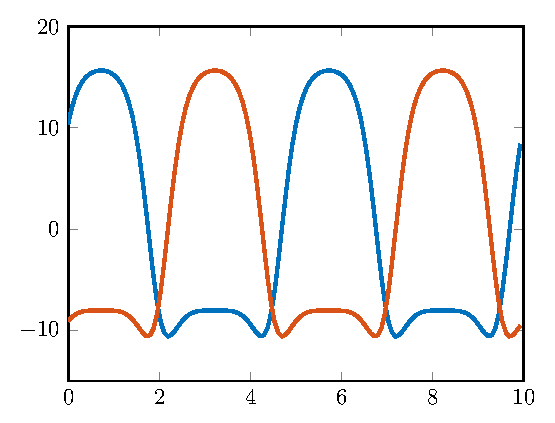
\includegraphics[width=\textwidth]{figures/scft1.pdf}}
    \end{column}
    \begin{column}{0.5\textwidth}
        \uncover<3->{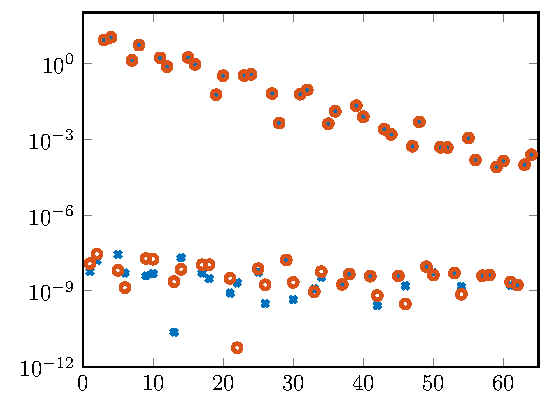
\includegraphics[width=\textwidth]{figures/scft2.pdf}}
    \end{column}
    \end{columns}
\end{frame}

\begin{frame}[t]
    \frametitle{Example}

    And now the same with $f = 1/3$.

    \vfill
    \begin{columns}
    \begin{column}{0.5\textwidth}
        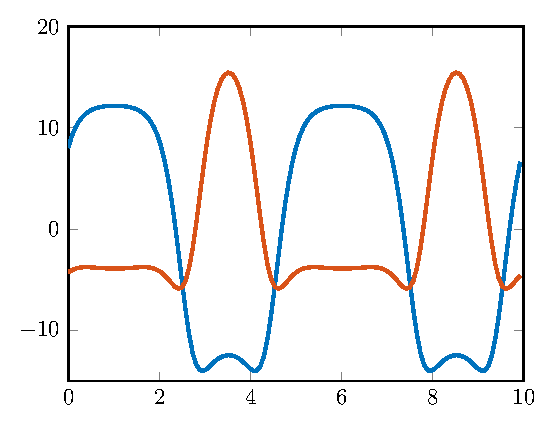
\includegraphics[width=\textwidth]{figures/scft_example2_fields.pdf}
    \end{column}
    \begin{column}{0.5\textwidth}
        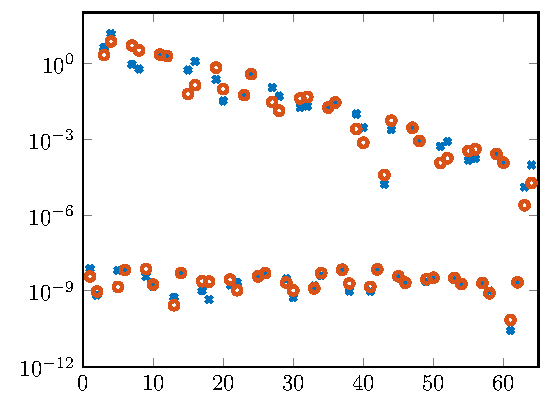
\includegraphics[width=\textwidth]{figures/scft_example2_fourier_coeffs.pdf}
    \end{column}
    \end{columns}
\end{frame}

\begin{frame}[t]
    \frametitle{What's striking?}

    \begin{itemize}
        \item External fields often exhibit regularity and some kind of symmetry.
    \end{itemize}

    \vfill

    \begin{columns}
        \begin{column}{0.5\textwidth}
            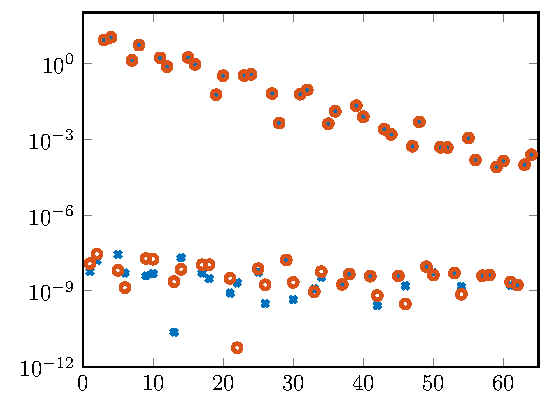
\includegraphics[width=\textwidth]{figures/scft2.pdf}
        \end{column}
        \begin{column}{0.5\textwidth}
            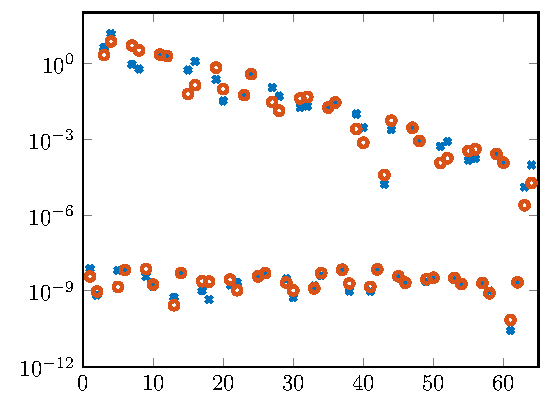
\includegraphics[width=\textwidth]{figures/scft_example2_fourier_coeffs.pdf}
        \end{column}
    \end{columns}

    \onslide<2->
    Maybe this can be used as a leverage point for a model reduction by only considering the functions with significant coefficients
    $\rightarrow$ model reduction by reduced basis method.
\end{frame}

\begin{frame}[t]
    \frametitle{Intermission: Reduced Basis Method}
    \framesubtitle{Preliminaries}

    Given a parametric variational problem
    \begin{equation}
        b(u, v; \bm \sigma) = f(v; \bm \sigma), \qquad u \in \mathcal X, v \in \mathcal Y,
    \end{equation}
    where
    \begin{itemize}
        \item $\mathcal X, \mathcal Y$ are Hilbert spaces,
        \item $\mathcal P \subset \mathbb{R}^{P}$, $P \in \mathbb{N}$, is a closed parameter space,
        \item $b \colon \mathcal X \times \mathcal Y \times \mathcal P \to \mathbb{R}$ is a parametric continuous bilinear form,
        \item $f \colon \mathcal Y \times \mathcal P \to \mathbb{R}$ is a parametric continuous linear functional.
    \end{itemize}

    \onslide<2>
    Let's assume
    \begin{equation}
        \beta(\bm \sigma) := \infsup{u \in \mathcal X}{v \in \mathcal Y} \frac{b(u, v; \bm \sigma)}{\norm{u}_{\mathcal X}\norm{v}_{\mathcal Y}}  > 0 \qquad \text{for all } \bm \sigma \in \mathcal P.
    \end{equation}
    $+$ some minor assumptions $\Rightarrow$ for every $\bm \sigma \in \mathcal P$ exists an unique solution $u(\bm \sigma)$.
\end{frame}

\begin{frame}[t]
    \frametitle{Intermission: Reduced Basis Method}
    \framesubtitle{Basic idea}

    \onslide
    Let's assume we want to compute the solution $\bm \sigma \mapsto u(\bm \sigma)$ in real time or for lots of different parameters $\bm \sigma \in \mathcal P$
    $\rightarrow$ standard Galerkin methods are likely too slow!

    \begin{itemize}
        \item \onslide<2->Let $\mathcal M := \Set{ u(\bm \sigma) \given \bm \sigma \in \mathcal P }$.
        \item Depending on the properties of the variational problem, $\mathcal M$ is often a smooth manifold with low dimension.
        \item \onslide<3-> This can be used for model reduction: instead of $\mathcal X$ use $\mathcal M$ as the ansatz space!
    \end{itemize}

    \vfill

    \onslide<4->
    Further we won't use the continuous variational problem, but instead the \emph{truth} variational problem based on a high dimensional Galerkin method:
    \begin{equation}
        b(u, v; \bm \sigma) = f(v; \bm \sigma), \qquad u \in \mathcal X_{\mathcal N}, v \in \mathcal Y_{\mathcal N},
    \end{equation}
    with subspaces $\mathcal X_{\mathcal N} \subset \mathcal X$, $\mathcal Y_{\mathcal N} \subset \mathcal Y$.
\end{frame}

\begin{frame}[t]
    \frametitle{Intermission: Reduced Basis Method}
    \framesubtitle{Basic idea}

    The reduced basis method consists off two stages:

    \begin{itemize}
        \item \onslide<2-> \emph{Offline stage:} Construction of \enquote{optimal} reduced basis spaces $\mathcal X_{N} := \Set{u_{\mathcal N}(\bm \sigma_n) \given n = 1, \dots, N} \subset \mathcal M_{\mathcal N}$ and $\mathcal Y_{N} \subset \mathcal Y_{\mathcal N}$ with low dimension.
        \item \onslide<4-> \emph{Online stage:} Given a parameter $\bm \sigma \in \mathcal P$, compute the rb-solution $u_{N}(\bm \sigma)$ and a certified bound for the error $\norm{u_{N}(\bm \sigma) - u_{\mathcal N}(\bm \sigma)}_{\mathcal X}$ (both independent of $\mathcal N$).
    \end{itemize}
    \centering
    $\;$\\[-3.7em]
    \onslide<3-> 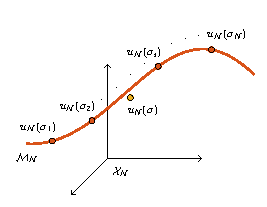
\includegraphics[width=0.58\textwidth]{figures/rb.pdf}
\end{frame}

\begin{frame}[t]
    \frametitle{Intermission: Reduced Basis Method}
    \framesubtitle{Certified error bound}
    Let $r_{N} \colon \mathcal Y_{\mathcal N} \times \mathcal P \to \mathbb{R}$ be the residual
    \begin{equation}
        r_{N}(v; \bm \sigma) := b(u_{\mathcal N}(\bm \sigma) - u_{N}(\bm \sigma), v; \bm \sigma) = f(v; \bm \sigma) - b(u_{N}(\bm \sigma), v; \bm \sigma).
    \end{equation}
    $\Rightarrow$ linear functional for every $\bm \sigma \in \mathcal P$.

    \onslide<2>
    Standard theorems leads to a posteriori error bound
    \begin{equation}
        \norm{u_{N}(\bm \sigma) - u_{\mathcal N}(\bm \sigma)}_{\mathcal X} \leq \frac{\norm{r_{N}(\blank; \bm \sigma)}_{\mathcal Y_{\mathcal N}'}}{\beta_{\mathrm{LB}}(\bm \sigma)} =: \Delta_{N}(\bm \sigma),
    \end{equation}
    where
    \begin{itemize}
        \item norm of the residual can be efficiently computed through Riesz representation theorem,
        \item $\beta_{\mathrm{LB}}(\bm \sigma)$ is a computable lower bound for $\beta(\bm \sigma)$.
    \end{itemize}
\end{frame}

\begin{frame}[t]
    \frametitle{Intermission: Reduced Basis Method}
    \framesubtitle{Inf-sup-constant}

    Problem: how to compute $\beta_{\mathrm{LB}}(\bm \sigma)$ efficiently?

    \vfill
    \onslide<2->
    Default is the so called successive constraint method.

    \begin{itemize}
        \item Reinterpret the calculation of $\beta(\bm \sigma)$ as an optimization problem
        \\$\rightarrow$ linear objective function, but feasible region in general not a convex polytope.
        \item \onslide<3->\emph{Offline stage:} Construct \enquote{optimal} lower and upper bounds for the feasible region.
        \item \onslide<4->\emph{Online stage:} Compute $\beta_{\mathrm{LB}}(\bm \sigma)$ through small linear program.
    \end{itemize}

    \vfill
\end{frame}

\begin{frame}[t]
    \frametitle{Intermission: Reduced Basis Method}
    \framesubtitle{Offline and online stage}

    Offline stage needs a discrete \enquote{training set} $\mathcal P_{\mathrm{train}} \subset \mathcal P$.\newline
    Iterative greedy scheme, start with random $\bm \sigma_{1} \in \mathcal P_{\mathrm{train}}$, $\mathcal X_{1} := \Set{u_{\mathcal N}(\bm \sigma_{1})}$:\\[0em]
    \onslide<2->
    \begin{enumerate}
        \item find $\bm \sigma_{N + 1} := \argmax_{\bm \sigma \in \mathcal P_{\mathrm{train}}} \Delta_{N}(\bm \sigma)$,
        \item set $\mathcal X_{N + 1} := \spn (\mathcal X_{N} \cup \Set{u_{\mathcal N}(\bm \sigma)})$,
        \item repeat until maximum in step 1 is smaller than a given tolerance.
    \end{enumerate}
    $\rightarrow$ computationally intensive part.
    \vfill

    \onslide<3->
    Online stage, given a $\bm \sigma \in \mathcal P$:\\[0em]
    \begin{enumerate}
        \item solve reduced basis system for $u_{N}(\bm \sigma) \in \mathcal X_{N}$,
        \item compute certified error bound $\Delta_{N}(\bm \sigma)$.
    \end{enumerate}
    $\rightarrow$ runtime depends only on low dimension $N$, not $\mathcal N$.
\end{frame}

\begin{frame}[t]
    \frametitle{Intermission: Reduced Basis Method}
    \framesubtitle{Examples}

    Typical results of the offline stage, one dimensional parameter space.

    \centering
    \includegraphics<1>[width=0.9\textwidth]{figures/1d_par_s_1.pdf}
    \includegraphics<2>[width=0.9\textwidth]{figures/1d_par_s_2.pdf}
    \includegraphics<3>[width=0.9\textwidth]{figures/1d_par_s_3.pdf}
    \includegraphics<4>[width=0.9\textwidth]{figures/1d_par_s_4.pdf}
\end{frame}

\begin{frame}[t]
    \frametitle{Intermission: Reduced Basis Method}
    \framesubtitle{Examples}

    And now a three dimensional parameter space.

    \centering
    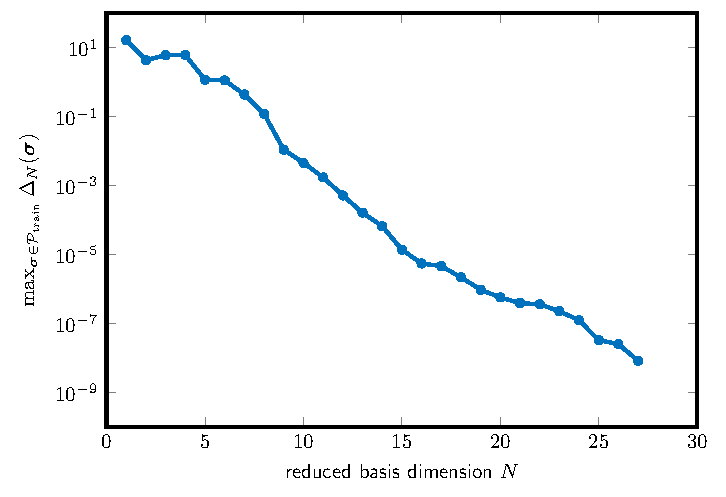
\includegraphics[width=0.9\textwidth]{figures/3dplot.pdf}
\end{frame}


\begin{frame}[t]
    \frametitle{Back to the SCFT}

    What we've already done:

    \begin{itemize}
        \item<1-> Derived a space-time variational formulation (STVP) of the MDE based on Bochner spaces.
        \item<2-> Replaced the fields $w_A, w_B$ with parametric functions
        \begin{equation}
            w(\bm \sigma) = \sum_{j = 1}^{N} \sigma_{j} \phi_{j},
        \end{equation}
        where $N \in \mathbb{N} \cup \Set{ \infty }$, $\bm \sigma \in [-1, 1]^{N}$ and $\phi_{j} \in L_{\infty}(\Omega)$, $j = 1, \dots, N$.
        \item<2-> Shown, that the solution of the STVP depends analytically on the parameters (given some restrictive sufficient conditions).
        \item<3-> Applied a Petrov-Galerkin method to solve the STVP.
        \item<3-> Experimented with the application of the reduced basis method on the STVP.
    \end{itemize}

\end{frame}

\begin{frame}[t]
    \frametitle{Back to the SCFT}

    Problems encountered so far:

    \begin{itemize}
        \item<1-> The fact that $\mathcal X \neq \mathcal Y$ complicates lots of things.
        \item<2-> Most suitable Petrov-Galerkin methods aren't unconditionally stable.
        \item<3-> Successive constraint method suffers from curse of dimensionality and is quite slow for more than a handful of parameters.
        \\ $\rightarrow$ a priori knowledge about field expansion functions required to obtain a small number of parameters.
    \end{itemize}

\end{frame}

\end{document}
